\documentclass[]{article}
\usepackage{lmodern}
\usepackage{amssymb,amsmath}
\usepackage{ifxetex,ifluatex}
\usepackage{fixltx2e} % provides \textsubscript
\ifnum 0\ifxetex 1\fi\ifluatex 1\fi=0 % if pdftex
  \usepackage[T1]{fontenc}
  \usepackage[utf8]{inputenc}
\else % if luatex or xelatex
  \ifxetex
    \usepackage{mathspec}
    \usepackage{xltxtra,xunicode}
  \else
    \usepackage{fontspec}
  \fi
  \defaultfontfeatures{Mapping=tex-text,Scale=MatchLowercase}
  \newcommand{\euro}{€}
\fi
% use upquote if available, for straight quotes in verbatim environments
\IfFileExists{upquote.sty}{\usepackage{upquote}}{}
% use microtype if available
\IfFileExists{microtype.sty}{%
\usepackage{microtype}
\UseMicrotypeSet[protrusion]{basicmath} % disable protrusion for tt fonts
}{}
\ifxetex
  \usepackage[setpagesize=false, % page size defined by xetex
              unicode=false, % unicode breaks when used with xetex
              xetex]{hyperref}
\else
  \usepackage[unicode=true]{hyperref}
\fi
\hypersetup{breaklinks=true,
            bookmarks=true,
            pdfauthor={Jonathan Werner},
            pdftitle={Bachelor thesis - Better accuracy of automatic lecture transcriptions by using context information from slide contents},
            colorlinks=true,
            citecolor=blue,
            urlcolor=blue,
            linkcolor=magenta,
            pdfborder={0 0 0}}
\urlstyle{same}  % don't use monospace font for urls
\usepackage{longtable,booktabs}
\usepackage{graphicx,grffile}
\makeatletter
\def\maxwidth{\ifdim\Gin@nat@width>\linewidth\linewidth\else\Gin@nat@width\fi}
\def\maxheight{\ifdim\Gin@nat@height>\textheight\textheight\else\Gin@nat@height\fi}
\makeatother
% Scale images if necessary, so that they will not overflow the page
% margins by default, and it is still possible to overwrite the defaults
% using explicit options in \includegraphics[width, height, ...]{}
\setkeys{Gin}{width=\maxwidth,height=\maxheight,keepaspectratio}
\setlength{\parindent}{0pt}
\setlength{\parskip}{6pt plus 2pt minus 1pt}
\setlength{\emergencystretch}{3em}  % prevent overfull lines
\providecommand{\tightlist}{%
  \setlength{\itemsep}{0pt}\setlength{\parskip}{0pt}}
\setcounter{secnumdepth}{5}

\title{Bachelor thesis - Better accuracy of automatic lecture transcriptions by
using context information from slide contents}
\author{Jonathan Werner}
\date{}
\usepackage[utf8]{inputenc}
\usepackage{hyperref}
\usepackage[all]{hypcap}

\usepackage{titlesec}
\newcommand{\sectionbreak}{\clearpage}

% Redefines (sub)paragraphs to behave more like sections
\ifx\paragraph\undefined\else
\let\oldparagraph\paragraph
\renewcommand{\paragraph}[1]{\oldparagraph{#1}\mbox{}}
\fi
\ifx\subparagraph\undefined\else
\let\oldsubparagraph\subparagraph
\renewcommand{\subparagraph}[1]{\oldsubparagraph{#1}\mbox{}}
\fi

\begin{document}
\maketitle

{
\hypersetup{linkcolor=black}
\setcounter{tocdepth}{3}
\tableofcontents
}
\newpage

\section*{Introduction}\label{introduction}
\addcontentsline{toc}{section}{Introduction}

Scannability is crucial for academic research: you have to be able to
quickly evaluate the usefulness of a given resource by skimming the
content and looking for the parts that are specifically relevant to the
task at hand.

The medium in which those resources are available is very centered on
textual representation. Spoken content, hereinafter called \emph{speech
media} (audio- or audiovisual media that mainly consists of spoken
language) doesn't make it possible to scan its contents. You are
``stabbing in the dark'' when looking for something specific in a medium
like this and have to consume it like a linear narrative.

This means that although lectures and conference talks are a central
element to science they are much more challenging and tedious to use for
research work.

Being able to a) efficiently search and b) look at the temporal
distribution of important keywords in a visually dense way would elevate
the usefulness of speech media in the scientific context immensely.

One approach to accomplish those goals is utilizing Automatic Speech
Recognition (ASR) to transcribe speech to text and also get timing
information for the recognized words. This makes it possible to derive
information about the density of given words at a given point of time in
the talk, which in turn allows to compute word occurence density maxima.
This opens up possibilities for compact visual representation of the
interesting keywords, thus allowing the user to scan.

The main challenge when using ASR for this task is the recognition
accuracy of technical terms. Most of them are not included in the
language models that are available as those are broad and generic so as
to optimize for accuracy over a wide topic spectrum. But when they are
not included into the language model they have a very small chance to be
correctly recognized at all.

So the usefulness of applying ASR with a generic language model to the
problem is very small, as the intersection of interesting keywords with
those technical terms that can not be recognized is very big.

The central goal of this thesis is to explore an approach to overcome
this problem. This approach consists of using words from lecture slides
or other notes to generate a lecture-specific language model. This is
then interpolated with a generic language model and being compared to
the `baseline' accuracy of the generic model.

\pagebreak

\subsection*{Structure of this thesis}\label{structure-of-this-thesis}
\addcontentsline{toc}{subsection}{Structure of this thesis}

The structure of this thesis is laid out as follows:

\begin{enumerate}
\def\labelenumi{(\arabic{enumi})}
\item
  \textbf{Research questions}

  I will state the research questions.
\item
  \textbf{Scientific Background}

  \begin{enumerate}
  \item
    I will start by giving an overview over the state of the art of ASR
    and the most prevalent approaches.
  \item
    I will explain the \emph{concepts} which are fundamental for the
    understanding of speech recognition.
  \item
    I will then examine the \emph{scientific work} that has been done on
    applying ASR to the problem of lectures transcriptions.
  \item
    Finally i will summarize the \emph{metrics} that have been used to
    assess the quality of the improvements in different approaches.
  \end{enumerate}
\item
  \textbf{Motivation}

  Here i will motivate why it is necessary to improve on the baseline
  performance of ASR in our context.

  I will talk about the role of keywords and technical terms and why
  they are not being detected and how that diminishes the usefulness of
  ASR for the purposes of scannability.
\item
  \textbf{Test data}

  I will use the openly available \emph{Open Yale Courses} (\emph{Open
  Yale Courses Website}, n.d.), which provide a diverse selection of
  audio and video recordings of university lectures at Yale,
  additionally supplying quality manual transcriptions and course notes
  or slides.

  I will present the chosen courses, their selection criteria and
  discuss the range of types of lecture material.
\item
  \textbf{The LM-Interpolation approach}

  \begin{enumerate}
  \item
    \textbf{Technical basis}

    I will introduce the open source speech recognition framework
    \emph{Sphinx 4}. This is the software that is used for performing
    the actual recognition.
  \item
    \textbf{Process overview}

    I will then give a overview of the design and architecture of our
    approach.
  \item
    \textbf{Implementation}

    Finally i will describe the technical implementation by which the
    lecture material is compiled into a specialized language model and
    recognition is performed using a \emph{interpolated} language model.
  \end{enumerate}
\item
  \textbf{Analysis}

  \begin{enumerate}
  \item
    \textbf{Methods}

    I will discuss how to analyze the results and develop metrics that
    assess how well the given goals are met with our approach. 
  \item
    \textbf{Analysis}

    I will then perform quantitative analysis on our test dataset with
    the metrics we developed before.
  \item
    \textbf{Discussion, Finding and Conclusions}

    I will discuss the findings and draw conclusions from the
    quantitative analysis concerning the effectiveness of our approach.
  \end{enumerate}
\item
  \textbf{Visualization for Scannability}

  I will present a prototype visualization method that uses the results
  from our approach to present a condensed representation of the keyword
  content from lectures with the goal of providing a quick, interactive
  way to search and scan speech media.
\item
  \textbf{Improvements, Open Ends}

  I will discuss possible improvements and open ends that were out of
  the scope of this thesis but would be interesting to explore further.
\item
  \textbf{Summary}

  I will end by summarizing the goals, the proposed approach, the design
  and implementation, the analysis and the results.
\end{enumerate}

\pagebreak

\section{Research questions}\label{research-questions}

The central research questions i want to investigate in this thesis can
be formulated as follows:

\begin{enumerate}
\def\labelenumi{(\arabic{enumi})}
\item
  When we apply ASR to university lectures, what is the advantage of
  using an approach that consists of creating a lecture-specific
  language model and interpolating it with a generic language model,
  given that we are interested in improving the recognition accuracy of
  \emph{interesting keywords} for the sake of searchability and
  scannability?
\item
  What metric is useful for quantifying this advantage?
\end{enumerate}

A secondary question is: How can we \emph{use} the results from our
approach to provide graphical interfaces for improving the users ability
to search and scan the given speech medium?

The exploration of this question will not be the center of this thesis,
but it will provide practical motivation for the results that the
exploration.

\section{Background}\label{background}

\subsection{The field of Automatic Speech
Recognition}\label{the-field-of-automatic-speech-recognition}

Automatic Speech Recognition (ASR) can be defined as the process by
which a computer maps an acoustic speech signal to text
(\emph{comp.speech Frequently Asked Questions}, n.d.).

Rabiner \& Juang (\hyperref[ref-rabiner]{1993}) date the first research
on ASR back to the early 1950s, when Bell Labs built a system for
single-speaker digit recognition. Since then the field has seen three
major approaches, which Marquard (\hyperref[ref-marquard]{2012})
summarizes as follows:

\begin{quote}
\begin{enumerate}
\def\labelenumi{\arabic{enumi}.}
\tightlist
\item
  The \emph{acoustic-phonetic approach} aimed to identify features of
  speech such as vowels directly through their acoustic properties, and
  from there build up words based on their constituent phonetic
  elements.
\end{enumerate}
\end{quote}

\begin{quote}
\begin{enumerate}
\def\labelenumi{\arabic{enumi}.}
\setcounter{enumi}{1}
\tightlist
\item
  The \emph{statistical pattern-recognition approach} measures features
  of the acoustic signal, and compares these to existing patterns
  established from a range of reference sources to produce similarity
  scores which may be used to establish the best match.
\end{enumerate}
\end{quote}

\begin{quote}
\begin{enumerate}
\def\labelenumi{\arabic{enumi}.}
\setcounter{enumi}{2}
\tightlist
\item
  \emph{Artificial intelligence (AI) approaches} have been used to
  integrate different types of knowledge sources (such as acoustic,
  lexical, syntactic, semantic and pragmatic knowledge) to influence the
  output from a pattern-recognition system to select the most likely
  match.
\end{enumerate}
\end{quote}

The most prevalent approach today is the \emph{statistical
pattern-recognition approach}, as it produces results with much higher
accuracy compared to the acoustic-phonetic approach. The use of Hidden
Markov Models (HMM) has been playing a key role in this approach, as it
allows recognizers to use a statistical model of a given pattern rather
than a fixed representation.

In the last years there has been a resurgence of AI approaches,
specifically \emph{deep learning approaches} (Hinton et al.,
\hyperref[ref-hinton2012deep]{2012}). The ASR paradigm we will use for
this thesis will be limited to the former, however.

\subsection{Dimensions of speech
recognition}\label{dimensions-of-speech-recognition}

There are three dimensions which serve to classify different
applications of speech recognition (\emph{comp.speech Frequently Asked
Questions}, n.d., Marquard (\hyperref[ref-marquard]{2012})):

\begin{enumerate}
\def\labelenumi{(\arabic{enumi})}
\item
  \textbf{Dependent vs.~independent}. Dependent recognition systems are
  developed to be used by one speaker, whereas independent systems are
  developed to be used by \emph{any} speaker of a particular type, i.e
  North-American speakers. \textbf{Adaptive} systems lie between those
  poles, they are able to adapt to a particular speaker through
  training.
\item
  \textbf{Small vs.~large vocabulary}. Small vocabularies contain only
  up to a few hundred words and might be modeled by an explicit grammar,
  whereas large vocabularies contain tens of thousands of words so as to
  be able to model general purpose spoken language over a variety of
  domains.
\item
  \textbf{Continuous vs.~isolated speech}. Isolated speech consists of
  single words that are spoken with pauses in between them, whereas
  continuous speech consists of words that are spoken in a connected
  way. Continuous speech is significantly more difficult to recognize,
  as it is a) more difficult to find the start and end of words and b)
  the pronunciation of words changes in relation to their surrounding
  words.
\end{enumerate}

With those three dimensions we can for example classify the application
areas command and control systems, dictation and lecture transcription
(Marquard, \hyperref[ref-marquard]{2012}):

\begin{longtable}[c]{@{}llll@{}}
\caption{Three application areas}\tabularnewline
\toprule
Application & Speaker & Vocabulary & Duration\tabularnewline
\midrule
\endfirsthead
\toprule
Application & Speaker & Vocabulary & Duration\tabularnewline
\midrule
\endhead
Dictation & Dependent & Large & Connected\tabularnewline
Command and control system & Independent & Small &
Isolated\tabularnewline
Lecture transcription & Independent & Large & Connected\tabularnewline
\bottomrule
\end{longtable}

The task of automatic lecture transcriptions can thus be characterized
as speaker-independent (SI) large continuous speech recognition (LVCSR).

\subsection{Concepts}\label{concepts}

Speech recognition in the \emph{statistical pattern-recognition
approach} paradigm has three major concepts necessary for its
understanding:

\begin{itemize}
\tightlist
\item
  phonemes and phonetic dictionaries
\item
  acoustic models (AM)
\item
  language models (LM)
\end{itemize}

\subsubsection{Phonemes}\label{phonemes}

A \emph{phoneme} is ``the smallest contrastive linguistic unit which may
bring about a change of meaning'' (Cruttenden,
\hyperref[ref-cruttenden2014gimson]{2014}, p. 43). They are the smallest
unit of sound in speech which are combined to form words. The word
\emph{sun} for example can be represented by the phonemes \texttt{/s/},
\texttt{/u/} and \texttt{/n/}; the word \emph{table} by \texttt{/t/},
\texttt{/a/} and \texttt{/bl/}.

A language together with a specific accent can be described by a set of
phonemes that it consists of. Figure \ref{phonemic-chart} uses symbols
from the International Phonetic Alphabet (IPA) to display the 44
phonemes that are being used in Received Pronunciation (RP), which is
regarded as the ``standard accent'' in the south of the United Kingdom
(Stevenson \& Waite, \hyperref[ref-stevenson2011concise]{2011}).

\begin{figure}[htbp]
\centering
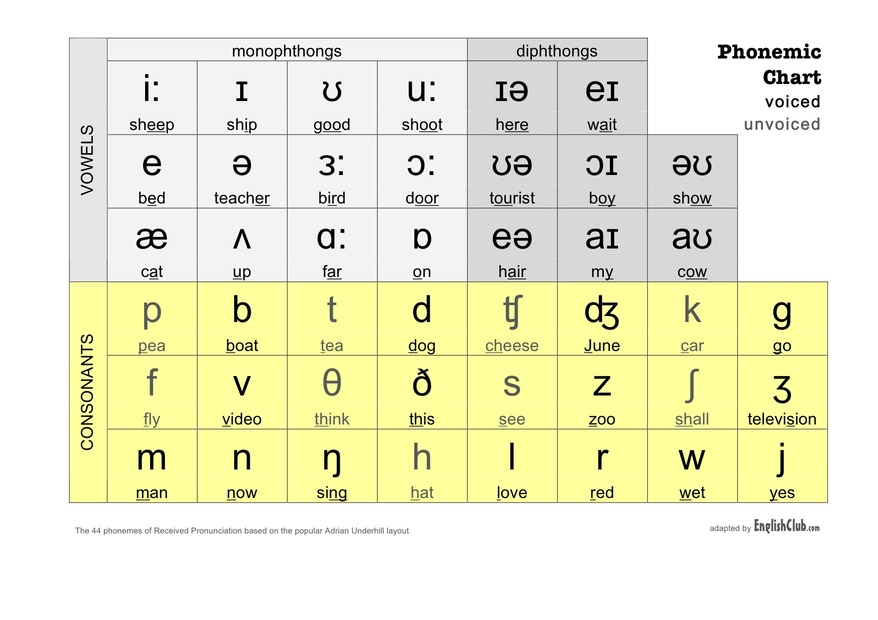
\includegraphics{images/phonemes_50.jpg}
\caption{Phonemic Chart representing 44 phonemes used in RP British
English\label{phonemic-chart}}
\end{figure}

To be able to use phonemes in software an ASCII representation is more
suitable. The standard for General American English is the
\emph{Arpabet}. Here each phoneme is mapped to one or two capital
letters. The digits \texttt{0}, \texttt{1} and \texttt{2} signify stress
markers: no stress, primary and secondary stress respectively. A
comparison of the IPA format and the arphabet format can be seen in
Figure \ref{arpabet}, an excerpt that just shows the
\emph{monophthongs}.\footnote{pure vowel sounds with relatively fixed
  articulation at the start and the end that don't glide towards a new
  position of articulation}

\begin{figure}[htbp]
\centering
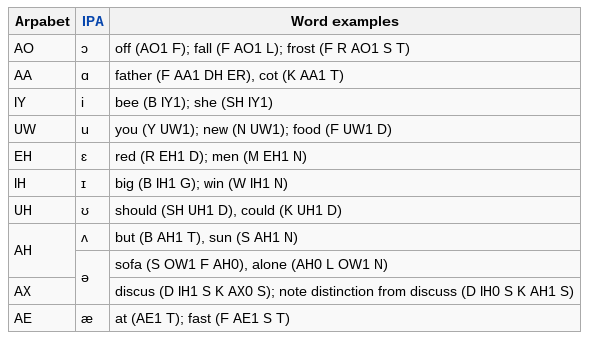
\includegraphics{images/arpabet.png}
\caption{Excerpt from the Arpabet (\emph{English Wikipedia Arpabet
article}, 2015 (accessed 22.8.15)) \label{arpabet}}
\end{figure}

\subsubsection{Phonetic dictionaries}\label{phonetic-dictionaries}

Phonetic dictionaries map words to one or multiple versions of phoneme
sequences.

A phonetic representation of a word is specified manually from the
knowledge how written words \emph{actually sound} when spoken.

An excerpt from the dictionary \texttt{cmudict-en-us.dict} (\emph{CMU
EN-US Pronouncing Dictionary (cmudict-en-us.dict)},
\hyperref[ref-cmuDict]{2015}) looks like this:

\begin{verbatim}
...
abdollah AE B D AA L AH
abdomen AE B D OW M AH N
abdomen(2) AE B D AH M AH N
abdominal AE B D AA M AH N AH L
abdominal(2) AH B D AA M AH N AH L
...
\end{verbatim}

The dictionary has 133.425 entries. In the general case only words that
are in the phonetic dictionary being used can be recognized during
speech recognition. \emph{Grapheme\footnote{``The smallest unit used in
  describing the writing system of a language'' Florian
  (\hyperref[ref-florian1996blackwell]{1996}), p.174}-to-Phoneme
converters} (G2P) however make it possible to get phoneme sequence
hypotheses for arbitrary words (that meaning arbitrary sequences of
graphemes). While those results are on average less accurate than
manually created variants, they play a vital role in texts with many
technical terms as those are often not part of phonetic dictionaries.

\subsubsection{Acoustic models}\label{acoustic-models}

An acoustic model (AM) describes the relation between an audio signal
and the probability that this signal represents a given phoneme.

Acoustic models are created by \emph{training} them on a \emph{corpus}
of audio recordings and matching transcripts. When being used in the
context of speaker-independent recognition, those models are trained
with a variety of speakers that represent a broad spectrum of the
language/accent that the acoustic model should represent.

During the \emph{decoding} phase the acoustic model and a phonetic
dictionary are used to match sequences of small audio ``slices'' to
possible phonemes and those phonemes to possible word sequence
hypotheses.

However, acoustic models alone are not sufficient for speech recognition
as they don't have the ``higher-level'' linguistic information necessary
to for example decide between homonyms and similar-sounding phrases such
as ``wreck a nice beach'' and ``recognize speech'' (Marquard,
\hyperref[ref-marquard]{2012}, p. 11). This information finally is
provided by \emph{language models}.

\subsubsection{Language Models}\label{language-models}

Language models (LM) guide and constrain the search process a speech
recognition system performs by assigning probabilities to sequences of
words. They are trained by applying statistical methods on a text
corpus. Analogous to acoustic models, generic language models use huge
text corpora with a broad variety of topics. It is however possible to
train language models on small and specialized text corpora, which is
the central technical foundation for the approach discussed in this
thesis.

The most commonly used form of language models are \emph{n-gram language
models}. In the context of a language model a \emph{n-gram} is a
sequence of \emph{n} words. 1-grams are called \emph{unigrams}, 2-grams
are called \emph{bigrams} and 3-grams are called \emph{trigrams}. A
\emph{n-gram language model} maps a set of \emph{n-grams} to
probabilities that they occur in a given piece of text.

A key idea in modelling language like this is the \emph{independence
assumption}, which says that the probability of a given word is only
dependent on the last \emph{n} - 1 words. This assumption significantly
decreases the statistical complexity and makes it thus computationally
feasible.

N-gram language models don't need to be constrained to one type of
n-gram. The \emph{Generic US English Generic Language Model}
(\emph{CMUSphinx US English Generic Language Model
(cmusphinx-5.0-en-us.lm)}, \hyperref[ref-cmuLm]{2015}) from CMUSphinx we
will use as the baseline for our approach for example consists of 1-, 2,
and 3-grams.

A toy example of a language model with 1- and 2-grams when represented
in \emph{ARPA}-format (as used by CMUSphinx) looks like follows
(\emph{CMUSphinx ARPA Language models}, 2015 (accessed 23.8.15)):

\begin{verbatim}
\data\
ngram 1=7
ngram 2=7

\1-grams:
-1.0000 <UNK>   -0.2553
-98.9366 <s>     -0.3064
-1.0000 </s>     0.0000
-0.6990 wood     -0.2553
-0.6990 cindy   -0.2553
-0.6990 pittsburgh      -0.2553
-0.6990 jean     -0.1973

\2-grams:
-0.2553 <UNK> wood
-0.2553 <s> <UNK>
-0.2553 wood pittsburgh
-0.2553 cindy jean
-0.2553 pittsburgh cindy
-0.5563 jean </s>
-0.5563 jean wood

\end\
\end{verbatim}

Here the first number in a row is the probability of the given n-gram in
\(log_{10}\) format. This means that the unigram \emph{wood} has a
probability of \(10^{-0.6990} \approx 0.2 = 20\%\) and the probability
of the words ``wood pittsburg'' occuring in sequence is
\(10^{-0.2553} \approx 0.55 = 55\%\) .

The optional third numeric column in a row is called \emph{backoff
weight}. Backoff weights make it possible to calculate n-grams that are
not listed by applying the formula

\begin{verbatim}
P( word_N | word_{N-1}, word_{N-2}, ...., word_1 ) =
P( word_N | word_{N-1}, word_{N-2}, ...., word_2 ) *
  backoff-weight( word_{N-1} | word_{N-2}, ...., word_1 )
\end{verbatim}

With the side condition that missing entries for
\texttt{word\_\{N-1\}\ \textbar{}\ word\_\{N-2\},\ ....,\ word\_1} are
replaced by \(1.0\).

So if the text to be recognized would contain the sequence ``wood
cindy'', which does not appear as a bigram in the LM, the probability
for this bigram could be calculated by
\texttt{P(wood\textbar{}cindy)\ =\ P(wood)\ *\ BWt(cindy)}.

Finally, the overall probability of a sentence with the words
\(w_1,...,w_n\) can be approximated as follows:

\[P(w_1,...,w_n) = \prod_{n=1}^m P(w_i \mid w_1,...w_{i-1})\]

An example approximation with a bigram model for the sentence ``I saw
the red house'' (\emph{English Wikipedia Language Model article}, 2015
(accessed 23.8.15)) represented as \(P(\text{I, saw, the, red, house})\)
would look like \[
  P(\text{I} \mid \langle s \rangle) \times
  P(\text{saw} \mid \text{I}) \times
  P(\text{the} \mid \text{saw}) \times
  P(\text{red} \mid \text{the}) \times
  P(\text{house} \mid \text{red}) \times
  P(\langle s \rangle \mid \text{house})
\]

\subsection{Work done on ASR for lecture
transcription}\label{work-done-on-asr-for-lecture-transcription}

I will now give an overview over the scientific work done on lecture
transcription, using Marquard (\hyperref[ref-marquard]{2012}) as a
guiding reference.

The research for speech recognition on lectures can be partitioned into
three general approaches: generalization approaches, specialization
approaches and approaches involving the user for manual correction and
improvements.

\subsubsection{Generalization
approaches}\label{generalization-approaches}

Generalization approaches try to create models that capture common
characteristics of lectures. Those characteristics include highly
spontaneous presentation style and ``strong coarticulation effects,
non-grammatical constructions, hesitations, repetitions, and filled
pauses'' (Yamazaki, Iwano, Shinoda, Furui, \& Yokota,
\hyperref[ref-yamazaki]{2007}). Glass, Hazen, Hetherington, \& Wang
(\hyperref[ref-glass]{2004}) note the ``colloquial nature'' of lectures
as well as the ``poor planning at the sentence level {[}and{]} higher
structural levels''.

The generalization approach has been applied on the acoustic model
level: Cettolo, Brugnara, \& Federico (\hyperref[ref-cettolo]{2004})
have examined adapting a generic acoustic model to account for
spontaneous speech phenomena (``filler sounds'').

While the a subfield of ASR called ``speaker diarization'' tries to
account for the interactivity between lecturers and students by
identifying multiple speakers, most research treats lectures as single
speaker events with the audience as background noise.

Generalization approaches at the language model level try to model
common linguistic traits of the lecture genre (this can be called the
``macro level''). Kato, Nanjo, \& Kawahara
(\hyperref[ref-kato2000]{2000}) investigate topic-independent language
modeling by creating a large corpus of text from lecture transcripts and
panel discussions and then removing topic-specific keywords.\footnote{In
  a second step they combine this generalization technique with a
  specialization technique by adapting the resulting LM with a
  lecture-specific language model by using preprint papers of a given
  lecture.}

\subsubsection{Specialization
approaches}\label{specialization-approaches}

Specialization approaches try to use context specific to a single
lecture (``meso level'') or parts of a single lecture (``micro
level''\footnote{The three levels are taken from Marquard
  (\hyperref[ref-marquard]{2012}).}).

Methods used for creating LMs from context information can be
categorized into two approaches: direct usage of lecture slides and
notes for the creation of LMs versus usage of ``derived'' data from
those materials. Deriving data by using keywords found in slides, using
them as web search query terms and using the found documents as the
basis for LM creation is explored in Munteanu, Penn, \& Baecker
(\hyperref[ref-munteanu]{2007}), Kawahara, Nemoto, \& Akita
(\hyperref[ref-kawahara08]{2008}) and Marquard
(\hyperref[ref-marquard]{2012}).

Using the whole text from lecture slides has been explored by Yamazaki
et al. (\hyperref[ref-yamazaki]{2007}). They compare the \emph{meso
level} with the \emph{micro level} by dynamically adapting the LM for
the speech corresponding to a particular slide. Kawahara et al.
(\hyperref[ref-kawahara08]{2008}) also examine dynamic local
slide-by-slide adaption and compare it to global topic adaption using
Probabilistic Latent Semantic Analysis (PLSA)\footnote{Latent Semantic
  Analysis is an approach to document comparison and retrieval which
  relies on a numeric analysis of word frequency and proximity. } and
web text collection, concluding that the last performs worse then the
former because of a worse orientation to topic words. .

\subsection{Metrics}\label{metrics}

\section{Test data}\label{test-data}

42 courses The test data i will use for evaluating our approach will be
from \emph{Open Yale Courses}\footnote{\url{http://oyc.yale.edu/}},
which is a selection of openly available lectures from Yale university.
It consists of 42 courses from 25 departments. Each course has about
20-25 sessions that have an average length of 50 minutes. Each lecture
is provided with good quality audio and video recordings, precise manual
transcripts and lecture material when available. Only about 20\% of the
lecture have lecture notes or slides at all and most materials from the
natural and formal science departments (physics, astronomics,
mathematics) consist of hand-written notes, making them unsuitable for
our approach. All talks are in English.

I have chosen the following lectures: (Department, Course, Lecture
Number - Title, abbreviation)

\begin{itemize}
\item
  \emph{Biomedical Engineering}: Frontiers of Biomedical Engineering, 1
  - What is Biomedical Engineering? (\texttt{biomed-eng-1})
\item
  \emph{Environmental Studies}: Environmental Politics and Law, 8 -
  Chemically Dependent Agriculture (\texttt{environmental-8})
\item
  \emph{Geology \& Geophysics}: The atmosphere, the ocean, and
  environmental change, 8 - Horizontal transport (\texttt{geology-8})
\item
  \emph{Philosopy}: Philosophy and the science of human nature, 8 -
  Flourishing and Detachment (\texttt{human-nature-8})
\item
  \emph{Psychology}: Introduction to Psychology, 14 - What Motivates Us:
  Sex (\texttt{psy-14})
\item
  \emph{Psychology}: Introduction to Psychology, 5 - What Is It Like to
  Be a Baby: The Development of Thought (\texttt{psy-5})
\end{itemize}

The main selection criterion here was topical diversity, with the
challenge that the majority of talks with computer-parsable notes was
from the humanities.

\subsection{Materials overview}\label{materials-overview}

The available material is very heterogeneous. I will now give an
overview with excerpts which will serve as a basis for examining later
if the quality and quantity of the supplied material is correlated with
the amount of improvement of our approach.

\texttt{geology-8} supplies a 2-page excercise sheet.

\begin{quote}
``Mars has a radius of 3.39 x 106 m and a surface gravity of 3.73 ms-2.
Calculate the escape velocity for Mars and the typical speed of a CO2
molecule (assume T = 250 K). How can Mars retain its CO2 atmosphere?
(Hint: the molecular weight of carbon dioxide is 44. Use the formulae
given in class.) {[}\ldots{}{]}''
\end{quote}

\texttt{biomed-eng-1} provides a 7-page glossary of technical terms.

\begin{quote}
``{[}\ldots{}{]} active transport - the transport of molecules in an
energetically unfavorable direction across a membrane coupled to the
hydrolysis of ATP or other source of energy

ATP (adenosine 5'-triphosphate) - a nucleotide that is the most
important molecule for capturing and transferring free energy in cells.
Hydrolysis of each of the two high-energy phosphoanhydride bonds in ATP
is accompanied by a large free-energy change (``G) of 7 kcal/mole

aquaporin -- a water channel protein which allows water molecules to
cross the cell membrane much more rapidly than through the phospholipid
bilayer {[}\ldots{}{]}"
\end{quote}

\texttt{human-nature-8} provides reading assignments for four books with
short summaries each.

\begin{quote}
``{[}A{]} Epictetus, The Handbook

Background information about the Stoic philosopher Epictetus (c. 50-130
CE) and his famous work Encheiridion (The Handbook) appears in Nicholas
White's introduction to our translation. White has also added footnotes
that explain points of potential confusion.

As the title indicates, The Handbook is intended as a tidy introduction
to a more complex philosophical outlook. It is written in an accessible
and engaging style.

The Stoic movement originated around 300 BCE and flourished for over
five hundred years. The Stoics believed that the external world is
deterministic: its state at any time is completely determined by its
prior states. So, they maintained, it is pointless to wish for things to
be different because to do so is to wish for something impossible. A
wise person would, therefore, accept whatever befalls them without
desiring that things go otherwise -- hence the English word `stoic.'
\end{quote}

\begin{quote}
Passages to focus on/passages to skim

I encourage you to read the text in full, at a steady reading pace.
{[}\ldots{}{]}"
\end{quote}

\texttt{psy-14/5} and \texttt{enviromental-8} provide
\textasciitilde{}10-page slides with a typical amount of text.

\subsubsection{Conclusion}\label{conclusion}

Only about 20\% of the courses have lecture material at all; only about
20\% of those actually have typical ``slides'' -- the rest provides
heterogenous other kinds of material. While it can not be inferred from
this dataset that this is a general condition, it nevertheless shows a
clear ``real-world'' disadvantage of an approach only relying on those
materials. We will look at the impact of the varying quality and
quantity in the analysis later.

\section{The LM-Interpolation
approach}\label{the-lm-interpolation-approach}

I will now describe the LM-Interpolation approach. The high level
overview looks like the following: we will use the open source speech
recognition framework Sphinx 4\footnote{Homepage:
  \url{http://cmusphinx.sourceforge.net/wiki/sphinx4:webhome}} as the
software for performing speech recognition. Sphinx 4 has a modular
architecture which allows specifying components of the whole process per
configuration. It provides multiple implementations of LMs\footnote{Overview:
  \url{http://cmusphinx.sourceforge.net/doc/sphinx4/edu/cmu/sphinx/linguist/language/ngram/LanguageModel.html}},
the default one being an ngram model.

It also provides an \texttt{InterpolatedLanguageModel}\footnote{Javadoc:
  \url{http://cmusphinx.sourceforge.net/doc/sphinx4/edu/cmu/sphinx/linguist/language/ngram/InterpolatedLanguageModel.html}}
(ILM), which allows you to specify multiple LMs and weights and
interpolate the probabilities for a given ngram from all models
probabilities (\(p = w_1*p_1 + w_2*p_2 + \ldots\) where \(w_n\) are the
weights (\(\sum_{i=1}^n(w_i) = 1\)) and \(p_i\) is the probability for a
given ngram in \(LM_i\)).

The ILM's use in our approach is to factor in the importance of
keywords. Those keywords have to be supplied in the form of an ngram
language model. For this we extract text content from the lecture
material, preprocess it and create an ngram LM from the resulting
corpus. Sphinx4 is then a) run with a generic english ngram LM only and
b) with the ILM configured to use the generic english LM and the keyword
language model in a 50/50 weighting. Finally the two resulting
transcriptions are compared with a selection of metrics.

As an example, the 1-gram \emph{sex} has a probability of 2.82\% in the
keyword model from \texttt{psy-14}, but a probability of 0.012\% in the
generic english LM.\footnote{(\emph{CMUSphinx US English Generic
  Language Model (cmusphinx-5.0-en-us.lm)}, \hyperref[ref-cmuLm]{2015})}
When applying 50/50 interpolation, the result is
\(2.82\%*0.5 + 0.012\%*0.5 = 1.416\%\), which is an increase by the
factor of \textasciitilde{}117 over the generic probability.

\subsection{Sphinx 4}\label{sphinx-4}

\subsection{Implementation}\label{implementation}

The pipeline is implemented with a collection of standalone command line
tools and a set of bash and python scripts\footnote{The source code is
  available here:
  \url{https://github.com/jonathanewerner/bachelor/tree/master/bin}.}.

The tasks are the following, in chronological order:

\begin{enumerate}
\def\labelenumi{\arabic{enumi}.}
\item
  \textbf{Prepare the input}

  \begin{itemize}
  \tightlist
  \item
    The audio file is converted into Sphinx 4 compatible format (16khz,
    16bit mono little-endian).
  \item
    A testcase folder with a given shortname (e.g. \texttt{psy-15}) is
    created in the \texttt{results}-directory\footnote{\url{https://github.com/jonathanewerner/bachelor/tree/master/results}}
    of the source code repository.
  \item
    The reference transcript, the material (PDF format is required) and
    the converted audio file are moved into a \texttt{resources}
    subfolder of the testcase folder.
  \end{itemize}
\item
  \textbf{Create a keyword LM from lecture material}

  \begin{itemize}
  \tightlist
  \item
    \texttt{pdftohtml\ -i\ -xml} is applied on the given material PDF.
    The XML output representation is input to
    \texttt{pdfreflow}\footnote{pdftohtml and pdfreflow are open source
      linux command line utilities}. Compared to the tool
    \texttt{pdftotext} the combination of these 2 tools preserves
    paragraphs correctly, whereas \texttt{pdftotext} represents each
    line break in the input PDF as a new paragraph in the output text
    file. This is a significant disadvantage for the LM creation step,
    as a newline in the input file there has the semantic ``end of
    sentence'' -- so that a sentence split into 4 lines by
    \texttt{pdftotext} would count as 4 sentences in the LM.
  \item
    The HTML output from \texttt{pdfreflow} is filtered by taking only
    relevant HTML-tags such as \texttt{\textless{}p\textgreater{}}'s
    (paragraphs) and \texttt{\textless{}blockquote\textgreater{}}'s,
    further improving the content-to-noise ratio.
  \item
    The resulting text is then preprocessed for optimal compatibility
    with the LM creation tool by removing punctuation and superfluous
    whitespace\footnote{I use a combination of command line text
      processing (sed) and a perl script from Stephen Marquard here.}.
  \item
    The resulting corpus is input to \texttt{estimate-ngram}, a LM
    creation tool from the MIT Language Modeling Toolkit\footnote{\url{https://code.google.com/p/mitlm/wiki/EstimateNgram}}
    (MITLMT).
  \end{itemize}
\item
  \textbf{Convert transcript to reference corpus}

  The transcript from Open Yale is supplied as HTML. We apply processing
  steps to transform it to a corpus ready to be consumed by the WER
  analysis tool (no punctuation, all lowercase). As these are specific
  to just the format chosen by Open Yale Courses, the details are
  omitted, as they have no general use.
\item
  \textbf{Run Sphinx 4 in baseline and interpolated mode}

  \texttt{bin/sphinx-interpolated.py}\footnote{\url{https://github.com/jonathanewerner/bachelor/blob/master/bin/sphinx-interpolated.py}}
  supplies a wrapper for interfacing with Sphinx 4. The Java API of
  Sphinx 4 is exposed for command line usage by a a JAR package which
  bundles the Sphinx 4 libraries and a small Main class. This class uses
  command line arguments supplied from
  \texttt{bin/sphinx-interpolated.py} to correctly configure Sphinx 4
  and start the actual recognition.

  Each testcase folder has a configuration file which specifies which
  models the test run should use:

\begin{verbatim}
  {
    "acousticModelPath": "en-new/cmusphinx-en-us-5.2",
    "dictionaryPath": "en-new/cmudict-en-us.dict",

    "languageModelPath": "en-new/cmusphinx-5.0-en-us.lm",
    "keywordModelPath": "model.lm",
    "g2pModelPath": "en-new/en_us_nostress/model.fst.ser",

    "resultsFolder": "biomed-eng-1"
  }
\end{verbatim}

  \texttt{bin/sphinx-interpolated.py} interprets the ``global'' models
  relative to the repository root-folder \texttt{models}, the
  \texttt{resultsFolder} relative to the root folder \texttt{results}
  and the \texttt{keywordModelPath} relative to the
  \texttt{resultsFolder}. It then supplies the absolute paths to the
  JAR. It also supplies absolute output file paths for the transcription
  result and transcription word timings results.

  This setup ensures reproducible results, as the environment of a given
  testcase is exactly specified (as long as the same binaries and script
  versions are assumed).

  \texttt{bin/sphinx-interpolated.py} can now be used to run the
  baseline or/and interpolated version.
\item
  \textbf{Analyze and compare the results}

  Finally the results from the two recognition runs are analyzed and
  compared by running
  \texttt{bin/hotword-analyze\ \textless{}testcase\ folder\ name\textgreater{}}.
  This performs two things: a) WER comparison and metrics generation and
  b) keyword visualization.

  5.1 \emph{WER comparison and metrics generation}

  This first calls \texttt{bin/wer.py}\footnote{\texttt{wer.py} has been
    adapted from
    \url{http://progfruits.blogspot.de/2014/02/word-error-rate-wer-and-word.html}}
  on each run, which will calculate the WER and show a summary of
  substituted (SUB), inserted (INS) and deleted (DEL) words when
  comparing the reference (REF) to the hypothesis (HYP):

\begin{verbatim}
OP  | REF     | HYP
INS | ****    | this
INS | ****    | is
INS | ****    | that
OK  | this    | this
OK  | is      | is
OK  | a       | a
OK  | course  | course
SUB | a       | that
SUB | version | aversion
OK  | of      | of
OK  | which   | which
SUB | i've    | i
OK  | taught  | taught
INS | ****    | him
...
...
{'Sub': 1230, 'Ins': 674, 'WER': 0.316, 'Del': 324, 'Cor': 5492}
\end{verbatim}

  In a second step it compares the two WER result files with
  \texttt{bin/compare-wer.py}.

  The result is an HTML file with a) shows a WER comparison table and b)
  various statistical measures which will be explored later. The table
  (shown in Figure \ref{wer-comparison}) colors correctly recognized
  words as green and incorrect words as red. It also marks words that
  have been improved in the interpolated version with a green border and
  words that have been worsened with a red border.

  \begin{figure}[htbp]
  \centering
  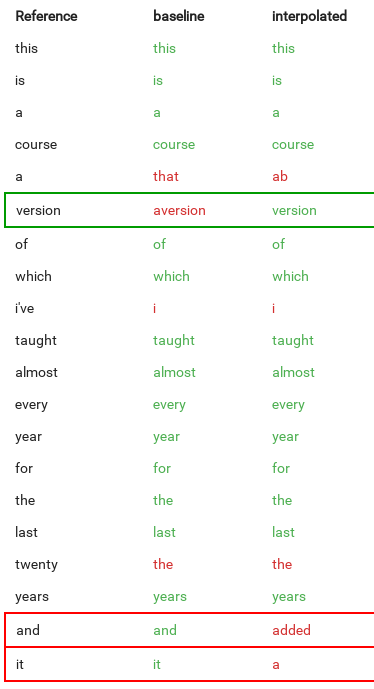
\includegraphics{images/wer-comparison_150.png}
  \caption{WER comparison\label{wer-comparison}}
  \end{figure}

  5.2 \emph{Keyword visualization}

  Data from the reference and the recognition results is compiled into a
  format suitable for consumption by a visualisation module, which will
  be discussed in depth further down in the chapter ``Visualization for
  Scannability''.
\end{enumerate}

All intermediate steps from the pipeline are represented as files in the
testcase folder. Table \ref{files} gives an overview of the files
created by each pipeline step.

\begin{longtable}[c]{@{}ll@{}}
\caption{File results of a testcase run\label{files}}\tabularnewline
\toprule
File & Description\tabularnewline
\midrule
\endfirsthead
\toprule
File & Description\tabularnewline
\midrule
\endhead
\textbf{Step 1: Prepare the input} &\tabularnewline
\texttt{resources/audio.mp3} & original audio\tabularnewline
\texttt{resources/audio.wav} & converted audio\tabularnewline
\texttt{resources/slides.pdf} & lecture material\tabularnewline
\texttt{resources/transcript.html} & lecture transcript\tabularnewline
\texttt{config.json} & run configuration\tabularnewline
&\tabularnewline
\textbf{Step 2: Create a keyword LM} &\tabularnewline
\texttt{slides.corpus.txt} & lecture material corpus\tabularnewline
\texttt{model.lm} & keyword LM\tabularnewline
&\tabularnewline
\textbf{Step 3: Convert reference to corpus} &\tabularnewline
\texttt{reference.corpus.txt} & reference transcription
corpus\tabularnewline
\texttt{reference\_wordcounts.json} & reference transcription word
counts\footnote{They are needed for the visualization later.}\tabularnewline
&\tabularnewline
\textbf{Step 4: Run Sphinx 4} &\tabularnewline
\texttt{sphinx\_log\_baseline.txt} & Sphinx 4 logging
output\tabularnewline
\texttt{sphinx\_log\_interpolated.txt} &\tabularnewline
\texttt{sphinx\_result\_baseline.txt} & Sphinx 4
transcription\tabularnewline
\texttt{sphinx\_result\_interpolated.txt} &\tabularnewline
\texttt{sphinx\_word\_times\_baseline.txt} & Sphinx 4 word
times\tabularnewline
\texttt{sphinx\_word\_times\_interpolated.txt} &\tabularnewline
&\tabularnewline
\textbf{Step 5.1: WER comparison / metrics generation} &\tabularnewline
\texttt{results.json} & run metrics in json format\footnote{This eases
  parsability for aggregating multiple testcase results later.}\tabularnewline
\texttt{wer\_baseline.txt} & WER table / metrics\tabularnewline
\texttt{wer\_interpolated.txt} &\tabularnewline
\texttt{wer\_comparison.html} & rich WER comparison +
metrics\tabularnewline
&\tabularnewline
\textbf{Step 5.2: Keyword visualization} &\tabularnewline
\texttt{cloud\_baseline.json} & data representation for
visualization\tabularnewline
\texttt{cloud\_interpolated.json} &\tabularnewline
\bottomrule
\end{longtable}

\section{Analysis}\label{analysiss}

\section*{References}\label{references}
\addcontentsline{toc}{section}{References}

\hyperdef{}{ref-cettolo}{\label{ref-cettolo}}
Cettolo, M., Brugnara, F., \& Federico, M. (2004). Advances in the
automatic transcription of lectures. In \emph{Acoustics, speech, and
signal processing, 2004. proceedings.(ICASSP'04). iEEE international
conference on} (Vol. 1, pp. I--769). IEEE.

\hyperdef{}{ref-cmuDict}{\label{ref-cmuDict}}
\emph{CMU EN-US Pronouncing Dictionary (cmudict-en-us.dict)}. (2015).
\url{https://github.com/cmusphinx/sphinx4/blob/master/sphinx4-data/src/main/resources/edu/cmu/sphinx/models/en-us/cmudict-en-us.dict}.

\hyperdef{}{ref-cmuArpa}{\label{ref-cmuArpa}}
\emph{CMUSphinx ARPA Language models}. (2015 (accessed 23.8.15)).
\url{http://cmusphinx.sourceforge.net/wiki/sphinx4:standardgrammarformats}.

\hyperdef{}{ref-cmuLm}{\label{ref-cmuLm}}
\emph{CMUSphinx US English Generic Language Model
(cmusphinx-5.0-en-us.lm)}. (2015).
\url{http://sourceforge.net/projects/cmusphinx/files/Acoustic\%20and\%20Language\%20Models/US\%20English\%20Generic\%20Language\%20Model/}.

\hyperdef{}{ref-cmufaq}{\label{ref-cmufaq}}
\emph{comp.speech Frequently Asked Questions}. (n.d.).
\url{http://www.speech.cs.cmu.edu/comp.speech/Section6/Q6.1.html}.

\hyperdef{}{ref-cruttenden2014gimson}{\label{ref-cruttenden2014gimson}}
Cruttenden, A. (2014). \emph{Gimson's pronunciation of English}.
Routledge.

\hyperdef{}{ref-wikiArpabet}{\label{ref-wikiArpabet}}
\emph{English Wikipedia Arpabet article}. (2015 (accessed 22.8.15)).
\url{https://en.wikipedia.org/wiki/Arpabet}.

\hyperdef{}{ref-wikiLM}{\label{ref-wikiLM}}
\emph{English Wikipedia Language Model article}. (2015 (accessed
23.8.15)). \url{https://en.wikipedia.org/wiki/Language_model}.

\hyperdef{}{ref-florian1996blackwell}{\label{ref-florian1996blackwell}}
Florian, C. (1996). The Blackwell encyclopedia of writing systems.
\emph{Oxford: Blackwell}.

\hyperdef{}{ref-glass}{\label{ref-glass}}
Glass, J., Hazen, T. J., Hetherington, L., \& Wang, C. (2004). Analysis
and processing of lecture audio data: Preliminary investigations. In
\emph{Proceedings of the workshop on interdisciplinary approaches to
speech indexing and retrieval at hLT-nAACL 2004} (pp. 9--12).
Association for Computational Linguistics.

\hyperdef{}{ref-hinton2012deep}{\label{ref-hinton2012deep}}
Hinton, G., Deng, L., Yu, D., Dahl, G. E., Mohamed, A.-r., Jaitly, N.,
Senior, A., et al. (2012). Deep neural networks for acoustic modeling in
speech recognition: The shared views of four research groups.
\emph{Signal Processing Magazine, IEEE}, \emph{29}(6), 82--97. IEEE.

\hyperdef{}{ref-kato2000}{\label{ref-kato2000}}
Kato, K., Nanjo, H., \& Kawahara, T. (2000). Automatic transcription of
lecture speech using topic-independent language modeling. In \emph{Sixth
international conference on spoken language processing}.

\hyperdef{}{ref-kawahara08}{\label{ref-kawahara08}}
Kawahara, T., Nemoto, Y., \& Akita, Y. (2008). Automatic lecture
transcription by exploiting presentation slide information for language
model adaptation. In \emph{Acoustics, speech and signal processing,
2008. iCASSP 2008. iEEE international conference on} (pp. 4929--4932).
IEEE.

\hyperdef{}{ref-marquard}{\label{ref-marquard}}
Marquard, S. (2012). Improving searchability of automatically
transcribed lectures through dynamic language modelling. University of
Cape Town.

\hyperdef{}{ref-munteanu}{\label{ref-munteanu}}
Munteanu, C., Penn, G., \& Baecker, R. (2007). Web-based language
modelling for automatic lecture transcription. In \emph{INTERSPEECH}
(pp. 2353--2356).

\hyperdef{}{ref-openyale}{\label{ref-openyale}}
\emph{Open Yale Courses Website}. (n.d.). \url{http://oyc.yale.edu/}.

\hyperdef{}{ref-rabiner}{\label{ref-rabiner}}
Rabiner, L., \& Juang, B.-H. (1993). Fundamentals of speech recognition.
Prentice hall.

\hyperdef{}{ref-stevenson2011concise}{\label{ref-stevenson2011concise}}
Stevenson, A., \& Waite, M. (2011). \emph{Concise Oxford English
Dictionary: Book \& CD-ROM Set}. Oxford University Press.

\hyperdef{}{ref-yamazaki}{\label{ref-yamazaki}}
Yamazaki, H., Iwano, K., Shinoda, K., Furui, S., \& Yokota, H. (2007).
Dynamic language model adaptation using presentation slides for lecture
speech recognition. \emph{Proc. INTERSPEECH 2007}, 2349--2352.

\end{document}
